\chapter{Opis struktury projektu}
\section{Wykorzystane technologie i narzędzia}
Projekt został zrealizowany w języku C\# jako aplikacja konsolowa, wykorzystująca platformę .NET (np. .NET 6.0 lub nowszy). Dane przechowywane są w prostych plikach tekstowych, co umożliwia łatwy odczyt i zapis informacji bez konieczności stosowania skomplikowanej bazy danych. Do tworzenia aplikacji wykorzystano środowiska takie jak Visual Studio lub Visual Studio Code. Minimalne wymagania sprzętowe to komputer z systemem Windows, Linux lub macOS, procesor o częstotliwości minimum 2 GHz oraz minimum 2 GB pamięci RAM.

\section{Struktura projektu i hierarchia klas}
Projekt składa się z siedmiu głównych klas:
\begin{itemize}
    \item \textbf{Program} – klasa zawierająca metodę \texttt{Main()}, która uruchamia aplikację.
    \item \textbf{Sklep} – główna klasa zarządzająca logiką działania systemu; integruje operacje związane z magazynem, klientami oraz zamówieniami.
    \item \textbf{Magazyn} – klasa odpowiedzialna za przechowywanie i aktualizację informacji o produktach, wykorzystująca strukturę typu słownik.
    \item \textbf{Produkt} – klasa reprezentująca pojedynczy produkt (nazwa, cena).
    \item \textbf{Koszyk} – klasa umożliwiająca gromadzenie produktów wybranych do sprzedaży oraz obliczanie całkowitej ceny.
    \item \textbf{Klient} – klasa przechowująca dane klienta (imię, nazwisko, saldo portfela).
    \item \textbf{Zamowienie} – klasa rejestrująca informacje o dokonanych transakcjach (data, dane klienta, lista zakupionych produktów).
\end{itemize}

\subsection{Diagram klas}
Poniżej przedstawiono diagram klas, który ilustruje hierarchię oraz relacje między poszczególnymi modułami systemu. Diagram ten prezentuje strukturę projektu w sposób graficzny, ukazując główne klasy, ich funkcje oraz wzajemne zależności. W diagramie uwzględniono takie elementy jak klasa \texttt{Program} – punkt wejścia do aplikacji, klasa \texttt{Sklep} odpowiedzialna za koordynację wszystkich operacji, a także klasy \texttt{Magazyn}, \texttt{Produkt}, \texttt{Koszyk}, \texttt{Klient} oraz \texttt{Zamowienie}, które reprezentują poszczególne elementy systemu. Klasa \texttt{Magazyn} zarządza listą produktów, \texttt{Produkt} definiuje właściwości pojedynczego artykułu, \texttt{Koszyk} umożliwia gromadzenie produktów wybranych do transakcji, natomiast \texttt{Klient} przechowuje dane o użytkownikach systemu, a \texttt{Zamowienie} rejestruje zakończone transakcje sprzedażowe. Taki diagram klas jest kluczowym narzędziem, które ułatwia zrozumienie architektury systemu oraz współdziałania jego modułów, co ma istotne znaczenie przy dalszym rozwijaniu i utrzymaniu projektu.

\begin{figure}[ht]
    \centering
    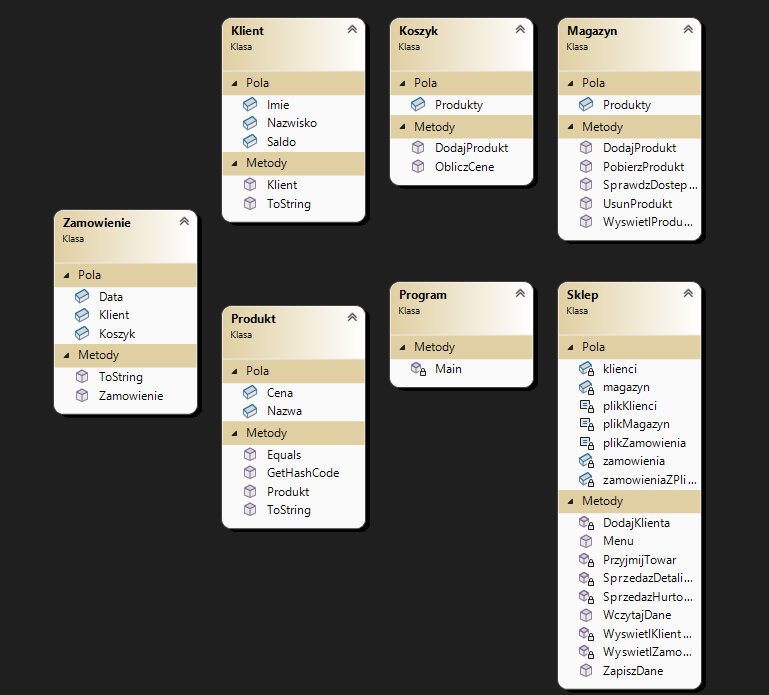
\includegraphics[width=0.9\linewidth]{figures/Hierarchia_klas.png}
    \caption{Diagram klas}
\end{figure}

\section{Zarządzanie danymi i baza danych}
Dane w systemie są przechowywane w trzech głównych plikach tekstowych:
\begin{itemize}
    \item \textbf{magazyn.txt} – zawiera informacje o produktach w formacie: nazwa; cena; ilość,
    \item \textbf{klienci.txt} – przechowuje dane klientów: imię; nazwisko; saldo,
    \item \textbf{zamowienia.txt} – zapisuje historię transakcji, zawierając datę, informacje o kliencie (lub informację o sprzedaży detalicznej) oraz listę zakupionych produktów.
\end{itemize}
Operacje CRUD (tworzenie, odczyt, aktualizacja, usuwanie) są realizowane poprzez odczytywanie danych z powyższych plików przy uruchomieniu systemu oraz zapisywanie zmian po zakończeniu pracy.


% ********** Koniec rozdziału **********
